\chapter{Theoretical Framework}

%TODO Introduction chapter

%Make clear that we are talking about Declarative Semantic knowledge

\section{Modal model of memory}

\begin{figure}
    \centering
    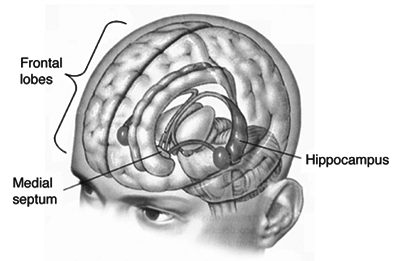
\includegraphics[width=0.5\textwidth]{img/brainareas.png}
    \caption{The brain areas mainly involved in storing and retrieving declarative knowledge \protect\cite{amnesia}}
    \label{fig:brainareas}
\end{figure}

Although the whole brain is involved in storing memories, the frontal lobes, medial septum and the hippocampus are the most prominent areas facilitating the process of memorising \cite{cognitivepsychology} (see figure~\ref{fig:brainareas}). The prefrontal regions are responsible for the creation and retrieval of memories, whereas the hipocampal and surrounding areas are responsible for permanent storage of these memories. Because of this dynamic, \citeA{modalmemory} conceived a modal theory of memory, displayed in figure~\ref{fig:modalmemory}. In this model, information is perceived as sensory input, and is then shortly stored in the sensory memory. If the perceiver has paid enough attention to the input, it is then transfered (or encoded) into short-term memory. When the input is strong enough, that is, rehearsed often enough within short term memory, it can be more permanently stored in long-term memory. If not, the input fades away from memory and is forgotten. When a memory exists in long-term memory, it has to be retrieved into short-term memory in order to be remembered and used.

This model was heavily influenced by developments in electrical engineering and computer sciences, and can be thought of as functioning like a complex computer, where data is written on a hard drive (the long-term memory), and can be used by first retrieving it into working memory (or short-term memory) and later be transferred to the hard drive again. However, the way the brain works is different from a computer in the sense that a brain has to put effort into memorising data, and that a brain forgets data over time. Therefore, instead of merely inputting the data, learning requires a more rigid approach.

\begin{figure}
    \centering
    
\includegraphics[width=0.5\textwidth]{img/modalmemory.png}
    \caption{The modal model of memory proposed by \protect\citeA{modalmemory}}
    \label{fig:modalmemory}
\end{figure}

\citeA{karpicke4} describes two seperate learning practices based on the modal model of memory, namely encoding and retrieval practices, where encoding practices are focused on meaningful encoding or construction of knowledge, and retrieval practiced are more focused on the reconstruction and rehearsal of knowledge. He states that both practices are essential to enhancing learning. Flashcards are a famous retrieval practice, emphasising drilling the same facts over and over again by means of pairs by association, whereas concept maps are known to be an encoding practice where the student has to connect diverse concepts within one topic by meaningful relations.

The following sections will elaborate on cognitive effects with regard to both encoding and retrieval practices, and relating them with their relevance to the effectiveness of concept mapping and flashcard systems respectively.

\section{Cognitive effects with regard to encoding practices}

The first step of memorisation is always encoding, because (logically speaking) it first has to be processed and encoded in either Short-Term or Long-Term Memory in order to be retrieved or used later on. After all, one cannot retrieve a memory which is not already there. It therefore is important to first acknowledge by which means knowledge is encoded, and in what kind of structure it is then stored.

\subsection{Spreading activation}

For centuries, a lot of metaphors describing memory characterised the brain as a room where a person could store physical things, such as a library filled with books or a storehouse with items \cite{roediger}.

Cajal found in the late 19th century that memories were patterns of electricity through neurons by means of synapses, which were thought to function like electrical wires \cite{longtermpotentiation}. 

\subsection{Schemata}

\subsection{Elaborative processing}

\subsection{Implications for concept mapping}

%Spreading activation
%Elaborative processing
%Schemata
%Constructionism

\section{Cognitive effects with regard to retrieval practices}

\subsection{Testing effect}



%Much of the successes attributed to retrieval practices are attributed towards the testing effect, the effect of retrieval strengthening memory more than extra opportunities for further encoding, even when the retrieval is only carried out internal only without any outward response \cite{microlearning}.

\subsection{Spacing effect}

The spacing effect is a well known effect occuring within paired-associate learning, and demonstrates that repeated items are better remembered when both occurences are seperated by other events or items than when they are presented in immediate succession \cite{verkoeijen, logan, siegel, xue, karpicke2}, which is demonstrated with diverse populations \cite{verkoeijen, logan}, under various learning conditions \cite{verkoeijen, logan}, and in both explicit and implicit memory tasks \cite{verkoeijen}. Items in immediate succession are called massed items, and items in seperated succession are called spaced items.

One can test the spacing effect either by using pure lists or mixed lists. When using pure lists, one compares the effect of learning a list containing only massed items with a list containing only spaced items, and using mixed lists one measures the effect of learning both massed items and spaced items in one list, comparing their individual retentions. \citeA{verkoeijen} states that the vast majority of studies are conducted using mixed lists and found that spaced items where consistenly better recalled than massed items, yet studies using pure lists are relatively rare and have produced contradictory outcomes. They conducted a study providing participants first with an all-massed list, then letting them write down as many words as they could remember, and repeat an identical procedure for an all-spaced list with a 2 minute break inbetween. They conducted this experiment with short-lagged spaced items (with 1-4 items in between) and long-lagged spaced items (with 4-13), and found only a spacing effect in the latter experiment. However, \citeA{wahlheim} adds to this that repetition is only increases when a student detects the repetition of an item, and therefore the lag should not be too long.

Two theories have been presented explaining this phenomenon, namely the contextual variability theory and the study-phase retrieval theory \cite{siegel}. The first theory entails that because context is not static but continuous, and that therefore spaced items are studied in a greater variety of contexts and therefore easier to recall in yet other contexts than massed items due to the so-called encoding-specificity principle \cite{cognitivepsychology}. This principle entails that the probability of recalling an item depends on the similarity of the context during the encoding. The study-phase retrieval theory entails that additional retrieval cues for the repetition of an item are generated by earlier occurences and their associated contexts being associated with the repeated item. These theories are not mutually exclusive \cite{siegel}.

\citeA{karpicke} conducted an experiment to test the effect of constant or varying lags between items have a significant effect on learning. They tested this by conducting a similar experiment to \citeA{verkoeijen}, however in this experiment they only tested pure lists with three different lag intervals to test for an absolute spacing effect, and for each lag interval category they tested for an expanding lag condition (where the lag would increase for the repetition of each next item), an equal lag condition (where the lag would remain constant) and a contracting lag condition (where the lag would decrease for the repetition of each next item) in order to test for a relative spacing effect. From their findings they confirmed the effect of absolute spacing, namely that longer gaps between items do have an effect on long-term retention, however they did not find a relative spacing effect. However, this has not been tested for spacing for longer intervals, such as intervals spanning multiple days or even weeks.

Although researchers have found at least an absolute spacing effect throughout multiple studies, students do not judge their learning to be improved by it, even when they demonstrated a significantly higher recall rate \cite{logan}.

\subsection{Power laws forgetting and learning}

\subsection{Implications for the flashcard system}
    %Pimsleur system
    %Leitner system
